\documentclass[t]{beamer}
\usetheme{Copenhagen}
\setbeamertemplate{headline}{} % remove toc from headers
\beamertemplatenavigationsymbolsempty

\usepackage{amsmath, tikz, pgfplots, tcolorbox, xcolor, array, bm}
\usetikzlibrary{calc}
\pgfplotsset{compat = 1.16}

\tikzstyle{input} = [circle, text centered, radius = 1cm, draw = black]
\tikzstyle{function} = [rectangle, text centered, minimum width = 2cm, minimum height = 1cm, draw = black]

\title{Transforming Functions}
\author{}
\date{}

\AtBeginSection[]
{
  \begin{frame}
    \frametitle{Objectives}
    \tableofcontents[currentsection]
  \end{frame}
}

\begin{document}

\begin{frame}{Parent Functions}
\begin{tabular}{cc}
    $y=x$   &   $y = x^2$   \\[11pt]
    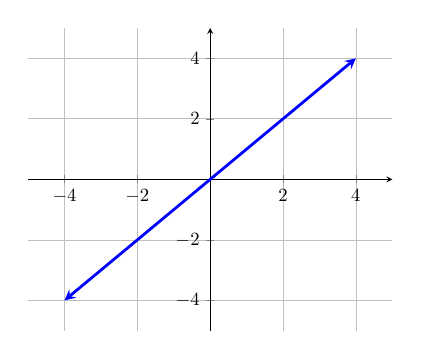
\begin{tikzpicture}[scale=0.675]
    \begin{axis}
    [
    xmin = -5,
    xmax = 5,
    ymin = -5,
    ymax = 5,
    grid,
    axis lines = middle
    ]
    \addplot[<->, >=stealth, color=blue, line width = 1.5, domain=-4:4] {x};
    \end{axis}
    \end{tikzpicture}
    &
    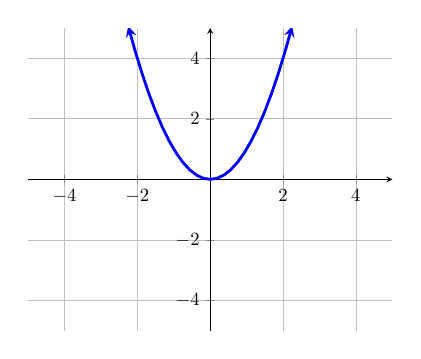
\begin{tikzpicture}[scale=0.675]
    \begin{axis}
    [
    xmin = -5,
    xmax = 5,
    ymin = -5,
    ymax = 5,
    grid,
    axis lines = middle
    ]
    \addplot[<->, >=stealth, color=blue, line width = 1.5, domain=-2.25:2.25] {x^2};
    \end{axis}
    \end{tikzpicture}
\end{tabular}
\end{frame}

\begin{frame}{Parent Functions}
\begin{tabular}{cc}
$y = x^3$   &   $y = |x|$   \\[11pt]
    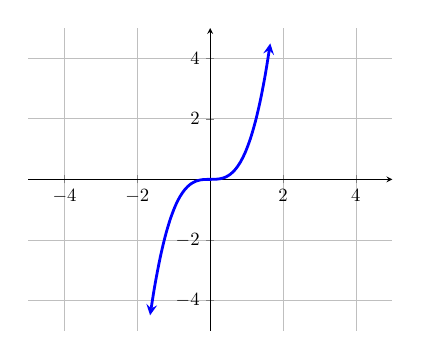
\begin{tikzpicture}[scale=0.675]
    \begin{axis}
    [
    xmin = -5,
    xmax = 5,
    ymin = -5,
    ymax = 5,
    grid,
    axis lines = middle
    ]
    \addplot[<->, >=stealth, color=blue, line width = 1.5, smooth, domain=-1.65:1.65] {x^3};
    \end{axis}
    \end{tikzpicture}
    &
    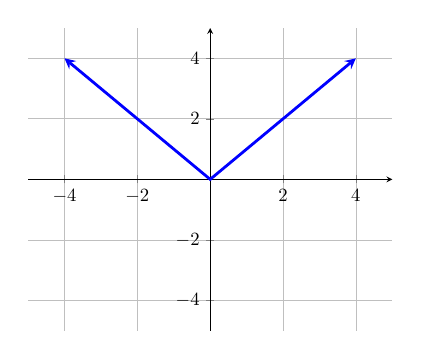
\begin{tikzpicture}[scale=0.675]
    \begin{axis}
    [
    xmin = -5,
    xmax = 5,
    ymin = -5,
    ymax = 5,
    grid,
    axis lines = middle
    ]
    \addplot[<->, >=stealth, color=blue, line width = 1.5, domain=-4:4] {abs(x)};
    \end{axis}
    \end{tikzpicture}
\end{tabular}
\end{frame}

\begin{frame}{Parent Functions}
\begin{tabular}{cc}
$y = \sqrt{x}$  &   $y = \sqrt[3]{x}$   \\[11pt]
    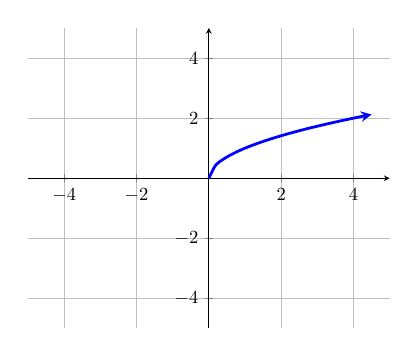
\begin{tikzpicture}[scale=0.67]
    \begin{axis}
    [
    xmin = -5,
    xmax = 5,
    ymin = -5,
    ymax = 5,
    grid,
    axis lines = middle
    ]
    \addplot[->, >=stealth, color=blue, line width = 1.5, smooth, domain=0:4.5] {sqrt(x)};
    \end{axis}
    \end{tikzpicture} 
    &   
    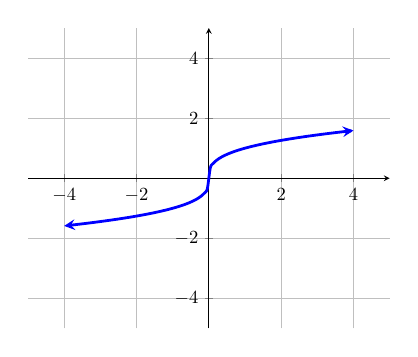
\begin{tikzpicture}[scale=0.67]
    \begin{axis}
    [
    xmin = -5,
    xmax = 5,
    ymin = -5,
    ymax = 5,
    grid,
    axis lines = middle
    ]
    \addplot[<->, >=stealth, color=blue, line width = 1.5, smooth, samples = 100, domain=-4:4] {x/abs(x)*abs(x)^(1/3)};
    \end{axis}
    \end{tikzpicture}
\end{tabular}
\end{frame}



\section{Perform vertical and horizontal shifts of functions}

\begin{frame}{$f(x) \pm d$}
\textsc{Investigation:}	\newline\\

For the function $f(x) = |x|$, examine the effects of
\[g(x) = |x| \pm d \]
where $d$ is a real number.
\end{frame}

\begin{frame}{Vertical shifts}
A \alert{vertical shift} (a.k.a. \alert{vertical translation}) moves each point on the graph either up or down by a given number of spaces.	\newline\\	\pause
\begin{center}

\setlength{\extrarowheight}{6pt}
\begin{tabular}{c|c|c}
\textbf{Equation}	&	\textbf{Shift Graph} & \textbf{Visually} \\ \hline
$f(x) + d$	& Up	& Add $d$ to $y$-coordinates	\\[6pt]	\hline
$f(x) - d$ & Down & Subtract $d$ from $y$-coordinates \\
\end{tabular}
\end{center}
\end{frame}

\begin{frame}{Example 1}
For each, list the parent function and indicate the vertical translation. \emph{Be specific}.	\newline\\	
(a) \quad $g(x) = x^2 + 3$	\newline\\	\pause
Parent function: $f(x) = x^2$	\newline\\	\pause
Transformation: Shift up 3 units
\end{frame}

\begin{frame}{Example 1}
(b) \quad $g(x) = x^3 - 2$	\newline\\	\pause
Parent function: $f(x) = x^3$	\newline\\	\pause
Transformation: Shift down 2 units
\end{frame}

\begin{frame}{Example 1}
(c) \quad $g(x) = |x| + 4.7$	\newline\\	\pause
Parent function: $f(x) = |x|$	\newline\\	\pause
Transformation: Shift up 4.7 units
\end{frame}

\begin{frame}{$f(x \pm c)$}
\textsc{Investigation:}	\newline\\

For the function $f(x) = |x|$, examine the effects of
\[g(x) = |x \pm c| \]
where $c$ is a real number.
\end{frame}

\begin{frame}{Horizontal shifts}
A \alert{horizontal shift} (a.k.a. \alert{horizontal translation}) moves each point on the graph either left or right by a given number of spaces.	\newline\\	\pause
\begin{center}
\setlength{\extrarowheight}{6pt}
\begin{tabular}{c|c}
\textbf{Equation}	&	\textbf{Shift Graph} \\ \hline
$f(x+c)$	& Left	\\[6pt]	\hline
$f(x-c)$ & Right \\
\end{tabular}
\end{center}
\vspace{8pt} \pause
{\color{blue}\textbf{Note:}} With horizontal shifts, the addition or subtraction is done \underline{inside} the function. \pause \newline\\

You will need to use ( ) for functions like $x^2$ and $x^3$.
\end{frame}

\begin{frame}{Example 2}
For each, list the parent function and indicate the horizontal translation. \emph{Be specific.}	\newline\\
(a) \quad $g(x) = (x-2)^2$	\newline\\	\pause
Parent function: $f(x) = x^2$ \newline\\	\pause
Transformation: Shift right 2 units
\end{frame}

\begin{frame}{Example 2}
(b) \quad $g(x) = |x+3|$	\newline\\	\pause
Parent function: $f(x) = |x|$ \newline\\	\pause
Transformation: Shift left 3 units
\end{frame}

\begin{frame}{Example 2}
(c) \quad $g(x) = \sqrt{x-6}$	\newline\\	\pause
Parent function: $f(x) = \sqrt{x}$ \newline\\	\pause
Transformation: Shift right 6 units
\end{frame}

\section{Perform vertical stretches and compressions of functions}

\begin{frame}{$a \cdot f(x)$}
\textsc{Investigation:}	\newline\\

For the function $f(x) = \sin x$, examine the effects of
\[g(x) = a \cdot \sin x \]
where $a > 1$ and also where $0 < a < 1$.
\end{frame}

\begin{frame}{Vertical Stretches and Compressions}
A \alert{vertical stretch} or \alert{vertical compression} is obtained by vertically pulling on (or vertically pressing on) the graph.	\newline\\	\pause

A vertical stretch pulls the points away from the $x$-axis, while a vertical compression pushes the points towards the $x$-axis. \newline\\ \pause

Algebraically, we obtain vertical stretches and compressions by multiplying the entire function by a positive value.
\end{frame}

\begin{frame}{Vertical Stretches and Compressions}
\begin{center}
\setlength{\extrarowheight}{6pt}
\begin{tabular}{c|c|c}
\textbf{Value of $\bm{a}$} & \textbf{Stretch or Compress?} & \textbf{Factor} \\ \hline
$a > 1$ & Stretch & $a$ \\[6pt] \hline
$0 < a < 1$ & Compression & $\frac{1}{a}$ \\
\end{tabular}
\end{center}
\pause \vspace{11pt}
Vertical stretches and compressions will multiply the $y$-coordinates  of the function by whatever the value of $a$ is.	\newline\\	\pause

\alert{\emph{Note:}} The factor is expressed as a value greater than 1.
\end{frame}

\begin{frame}{Example 3}
List the parent function and indicate if there is a vertical stretch or vertical compression. Then list the factor.	\newline\\
(a) \quad $g(x) = 2\sqrt{x}$	\newline\\	\pause
Parent function: $f(x) = \sqrt{x}$ \newline\\	\pause
Transformation: Vertical stretch by factor of 2
\end{frame}

\begin{frame}{Example 3}
(b) \quad $g(x) = 3.5\sqrt[3]{x}$	\newline\\	\pause
Parent function: $f(x) = \sqrt[3]{x}$ \newline\\	\pause
Transformation: Vertical stretch by factor of 3.5
\end{frame}

\begin{frame}{Example 3}
(c) \quad $g(x) = \dfrac{1}{3}x^2$	\newline\\	\pause
Parent function: $f(x) = x^2$ \newline\\	\pause
Transformation: Vertical compression by factor of 3
\end{frame}

\begin{frame}{Example 3}
(d) \quad $g(x) = \dfrac{2}{5}|x|$	\newline\\	\pause
Parent function: $f(x) = |x|$ \newline\\	\pause
Transformation: Vertical compression by factor of $\dfrac{5}{2}$
\end{frame}

\section{Perform reflections of functions across the x- and y-axes}

\begin{frame}{Reflections of Functions Across the x- and y-axes}
\textsc{Investigation:}	\newline\\
For the function $f(x) = \sqrt{x}$, examine the effects of
\[g(x) = -\sqrt{x} \]
\end{frame}

\begin{frame}{Reflections of Functions Across the x- and y-axes}
\textsc{Investigation:}	\newline\\
For the function $f(x) = \sqrt{x}$, examine the effects of
\[g(x) =\sqrt{-x} \]
\end{frame}

\begin{frame}{Reflections Across the x- and y-Axes}
When we multiply by $-1$, we reflect our graph across either the $x$-axis or the $y$-axis.	\newline\\	\pause
\begin{center}
\setlength{\extrarowheight}{6pt}
\begin{tabular}{c|c}
\textbf{Function} & \textbf{Reflect Across} \\ \hline
$-f(x)$ & $x$-axis \\[6pt] \hline
$f(-x)$ & $y$-axis
\end{tabular}
\end{center}
\end{frame}

\begin{frame}{Example 4}
List the parent function and indicate the axis it is reflected across. \newline\\
(a) \quad $g(x) = \sqrt[3]{-x}$	\newline\\	\pause
Parent function: $f(x) = \sqrt[3]{x}$ \newline\\ \pause
Transformation: Reflected across the $y$-axis
\end{frame}

\begin{frame}{Example 4}
(b) \quad $g(x) = -|x|$	\newline\\	\pause
Parent function: $f(x) = |x|$ \newline\\ \pause
Transformation: Reflected across the $x$-axis
\end{frame}

\section{Perform multiple transformations of functions}

\begin{frame}{Order of Multiple Transformations}
For multiple transformations, perform them in the following order:	\newline\\	\pause
\begin{enumerate}
\item<+-> Horizontal translations (shift left or right) \newline\\
\item<+-> Reflections \newline\\
\item<+-> Vertical stretches or compressions \newline\\ 
\item<+-> Vertical translations (shift up or down)	\newline\\
\end{enumerate}
\onslide<6->{{\color{blue}\textbf{Note}:} Steps 2 and 3 may be switched without penalty.}
\end{frame}

\begin{frame}{Example 5}
Determine the parent function and list all transformations done to it. Be specific.	\newline\\
(a) \quad $g(x) = -2\sqrt{x-3}$ \newline\\
\onslide<2->{Parent function: $f(x) = \sqrt{x}$} \newline\\
\onslide<3->{Shift right 3 units \quad $\sqrt{x-3}$} \newline\\
\onslide<4->{Reflect across $x$-axis \quad $-\sqrt{x-3}$} \newline\\
\onslide<5->{Vertical stretch by factor of 2 \quad $-2\sqrt{x-3}$}
\end{frame}

\begin{frame}{Example 5}
(b) \quad $g(x) = \frac{1}{2}(x+3)^2$ \newline\\
\onslide<2->{Parent function: $f(x) = x^2$} \newline\\
\onslide<3->{Shift left 3 units \quad $(x+3)^2$} \newline\\
\onslide<4->{Vertical compression by a factor of 2 \quad $\frac{1}{2}(x+3)^2$}
\end{frame}

\begin{frame}{Example 5}
(c) \quad $g(x) = |-x+2|+1$ \newline\\
\onslide<2->{Parent function: $f(x) = |x|$} \newline\\
\onslide<3->{Shift left 2 units \quad $|x+2|$} \newline\\
\onslide<4->{Reflect across $y$-axis \quad $|-x+2|$} \newline\\
\onslide<5->{Vertical shift up 1 unit \quad $|-x+2|+1$}
\end{frame}

\begin{frame}{Example 5}
(d) \quad $g(x) = -\dfrac{1}{5}(-x-7)^3-4$ \newline\\
\onslide<2->{Parent function: $f(x) = x^3$} \newline\\
\onslide<3->{Shift right 7 units \quad $(x-7)^3$} \newline\\
\onslide<4->{Reflect across $y$-axis \quad $(-x-7)^3$} \newline\\
\onslide<5->{Vertical compression by factor of 5 \quad $\frac{1}{5}(-x-7)^3$} \newline\\ 
\onslide<6->{Reflect across $x$-axis \quad $-\frac{1}{5}(-x-7)^3$} \newline\\
\onslide<7->{Vertical shift down 4 units \quad $-\frac{1}{5}(-x-7)^3-4$}
\end{frame}

\end{document}